\documentclass[a4paper, oneside]{book}
\usepackage[italian]{babel}
\usepackage[utf8]{inputenc}
\usepackage[a4paper,top=2.5cm,bottom=2.5cm,left=2cm,right=2cm]{geometry}
\usepackage{amssymb}
\usepackage{amsthm}
\usepackage{graphics}
\usepackage{amsfonts}
\usepackage{amsmath}
\usepackage{amstext}
\usepackage{engrec}
\usepackage{rotating}
\usepackage[safe,extra]{tipa}
\usepackage{multirow}
\usepackage{hyperref}
\usepackage{enumerate}
\usepackage{braket}
\usepackage{marginnote}
\usepackage{pgfplots}
\usepackage{cancel}
\usepackage{polynom}
\usepackage{booktabs}
\usepackage{enumitem}
\usepackage{algorithm}
\usepackage{algpseudocode}
\usepackage{framed}
\usepackage{pdfpages}
\usepackage{pgfplots}
\usepackage{fancyhdr}
\usepackage{caption}
\usepackage{subcaption}
\usepackage{setspace}
\usepackage{hyperref}
\pagestyle{fancy}
\fancyhead[L,RO]{\slshape \rightmark}
\fancyfoot[C]{\thepage}

\title{Causal Networks}
\author{Tommaso Ferrario (\href{https://github.com/TommasoFerrario18}{@TommasoFerrario18})\\\\
Telemaco Terzi (\href{https://github.com/Tezze2001}{@Tezze2001})}
\date{Ottobre 2024}

\pgfplotsset{compat=1.13}

\begin{document}

\maketitle
\newtheorem{teorema}{Teorema}
\newtheorem{dimostrazione}{Dimostrazione}
\newtheorem{definition}{Definition}
\newtheorem{esempio}{Esempio}
\newtheorem{osservazione}{Osservazione}
\newtheorem{note}{Note}
\newtheorem{corollario}{Corollario}
\tableofcontents
\renewcommand{\chaptermark}[1]{
    \markboth{\chaptername
        \ \thechapter.\ #1}{}}
\renewcommand{\sectionmark}[1]{\markright{\thesection.\ #1}}

\chapter{Potential outcomes}
In the following course we will use the following notation:
\begin{itemize}
    \item $X$ to denote the random variable representing the \textbf{treatment}
          assignment.
    \item $Y$ to denote the random variable representing the \textbf{outcome} of
          interest.
    \item $Z$ to denote a set of random variables representing \textbf{covariates}.
\end{itemize}

Also, we will use uppercase letters to denote random variables and lowercase
letters to denote their realizations.

\begin{definition}[Potential outcomes]
    $Y(x)$ denotes what your outcome would be, if you were to take treatment $X = x$.
\end{definition}
A \textbf{potential outcome} $Y(x)$ is distinct from the \textbf{observed outcome} $Y$ in that not
all potential outcomes are observed. But, all potential outcomes can potentially
be observed but we can't observe potential outcome of a decision that isn't made.

The actually observed outcome depends on the given value $x$ of treatment $X$.
The potential outcome is the value of $Y$ before making the decision of the
treatment $X=x$.

Up until now, we have been considering an individual. However, the population
consists of many individuals. Each individual is tipically associated with one or
more variables, referred to as covariates $Z$. We denote each individual using $i$
as as subscript.

\begin{definition}[Individual treatment effect]
    The individual treatment effect (ITE) for the $i^{th}$ individual
    is defined as the difference between the potential outcomes:
    \begin{equation}
        \tau_i \triangleq Y_i(1) - Y_i(0)
    \end{equation}

    The main different is that $Y(x)$ is a random variable because different individuals
    have different potential outcomes. Meanwhile, $Y_i(x)$ is a treated as a
    non-random variable because it is the potential outcome is deterministic, because
    it is conditioned by $i$-individual.
\end{definition}

\begin{note}
    If the individual treatment effect is different from zero, we can call it
    the \textbf{causal effect} of the treatment. Otherwise, we can call it the
    \textbf{no causal effect}.
\end{note}

\section{Fundamental problem of causal inference}
As we said before, it's impossible to observe all potential outcomes for a given
individual. Therefore, we can't observe the causal effect:
\begin{equation*}
    \tau_i \triangleq Y_i(1) - Y_i(0)
\end{equation*}

The potential outcome that you don't observe are known as \textbf{counterfactuals}.
So, a potential outcome $Y(x)$ doesn't become counterfactual until another
potential outcome $Y(x')$ is observed.

\begin{note}
    There are no counterfactuals or factuals until the outcome is observed.
\end{note}
\begin{definition}
    The \textbf{average treatment effect} (ATE) is obtained by taking an average
    over the individual treatment effects:
    \begin{equation}
        \tau \triangleq \mathbb{E}[\tau_i] = \mathbb{E}[Y_i(1) - Y_i(0)] = \mathbb{E}[Y(1) - Y(0)]
    \end{equation}
    where we recall that the average is over the individuals $i$ if $Y_i(x)$ is
    deterministic.
\end{definition}

The fundamental problem can be see as a missing data problem. Therefore, we cannot
compute directly the average treatment effect. We could be tempted to use the
associational difference:
\begin{equation}
    \mathbb{E}[Y|X = 1] - \mathbb{E}[Y|X = 0]
\end{equation}

Unfortunately, this is not true in general to compute the average treatment effect.
Because $\mathbb{E}[Y|X = 1] - \mathbb{E}[Y|X = 0]$ is an associational quantity,
while $\mathbb{E}[Y(1)] - \mathbb{E}[Y(0)]$ is a causal quantity.

In general, they are not equal due to the \textbf{confounding} effect of the covariates
$Z$. For example, using the representation in figure \ref{fig:confounding} we can
say that the covariate $Z$ confounds the effect of $X$ on $Y$, because of the
following path:
\begin{equation*}
    X \rightarrow Y \leftarrow Z
\end{equation*}

\begin{figure}[!ht]
    \centering
    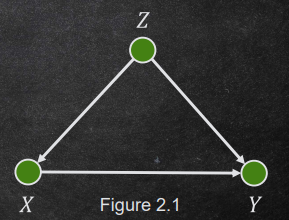
\includegraphics[width=0.35\textwidth]{img/confounding.png}
    \caption{Confounding effect of the covariate $Z$}
    \label{fig:confounding}
\end{figure}

We can consider average treatment effect equal to the associational difference
assuming the \textbf{ignorability} assumption.
\begin{definition}[Ignorability]
    The \textbf{ignorability} assumption states that the treatment assignment
    is random and independent of the potential outcomes:
    \begin{equation}
        Y(0), Y(1) \perp X
    \end{equation}
\end{definition}

Another name for this property is \textbf{exchangeability} because it can be
interpreted as we can exchange \textbf{treatment} and \textbf{control} groups without changing the
distribution of the potential outcomes.

In graphical sense, we can see the same structure of figure \ref{fig:confounding}
but without $Z \to X$ path.

We can distinguish between two types of ignorability:
\begin{itemize}
    \item \textbf{Mean ignorability}:
          \begin{equation*}
              \mathbb{E}[Y(1)|X = x]  =  \mathbb{E}[Y(1)]\ \ \ \
              \mathbb{E}[Y(0)|X = x]  =  \mathbb{E}[Y(0)] \ \forall x \in X
          \end{equation*}
    \item \textbf{Full ignorability}:
          \begin{equation*}
              (Y(1), Y(0))\perp X
          \end{equation*}
\end{itemize}
In general, mean ignorability is enough to compute the average
treatment effect.

This property is fundamental because it allows us to compute the average treatment
effect as the associational difference:
\begin{equation*}
    \tau \triangleq \mathbb{E}[Y(1) - Y(0)] = \mathbb{E}[Y|X = 1] - \mathbb{E}[Y|X = 0]
\end{equation*}

The assumption of ignorability allow us to identify causal effects. This can be
done reducing a causal expression to a purely statistical expression. We can
calculate the causal effect from just the observational distribution $P(X, Y, Z)$.

\begin{definition}[Identifiability]
    A causal quantity is identifiable if we can compute it from a purely statistical
    quantity.
\end{definition}

Unfortunately, the assumption of ignorability is completely unrealistic, confounding
is likely to happen in most data we observe. We can make the assumption of ignorability
more realistic by performing a \textbf{randomized experiment}, which force the treatment
$X$ to be cause randomly solving the problem of the confounding effect.

In observational data, it's unrealistic to assume that the groups are exchangeable.
However, if we control for relevant variables by conditioning, then maybe the groups
will be exchangeable.

\begin{definition}[Conditional exchangeability]
    The \textbf{conditional exchangeability} or \textbf{unconfoundeness} assumption
    states that the treatment assignment is the potential outcomes conditional
    on the covariates:
    \begin{equation}
        Y(0), Y(1) \perp X | Z
    \end{equation}
\end{definition}

Indeed, when conditioning on $Z$, non-causal associations between $X$ and $Y$ no
longer exists. Non-causal association is blocked by conditioning on $Z$.

This is the main assumption necessary for use the causal inference. We can now identify
the causal effect within levels of $Z$, just like we did with ignorability:
\begin{equation}
    \mathbb{E}[Y(1) - Y(0) | Z] = \mathbb{E}[Y(1)| Z] - \mathbb{E}[Y(0)| Z] =
    \mathbb{E}[Y|X = 1, Z] - \mathbb{E}[Y|X = 0, Z]
\end{equation}

If we want the marginal effect that we had before when assuming ignorability, we
can get that by simply marginalizing over $Z$ as follows:
\begin{equation}
    \mathbb{E}[Y(1) - Y(0)] = \mathbb{E}_Z[\mathbb{E}[Y(1) - Y(0) | Z]]
\end{equation}

\begin{definition}[Adjustment formula]
    Given the assumption of \textbf{unconfoundeness}, \textbf{positivity}, \textbf{consistency}, and \textbf{no interference},
    we can identify the average treatment effect as:
    \begin{equation}
        \tau = \mathbb{E}[Y(1) - Y(0)] = \mathbb{E}_Z[\mathbb{E}[Y(1) - Y(0) | Z]]
        = \mathbb{E}_Z[\mathbb{E}[Y|X = 1, Z] - \mathbb{E}[Y|X = 0, Z]]
    \end{equation}
\end{definition}

In the adjusted formula we moved from the assumption of ignorability to that
of unconfoundedness because it seems more realistic. However, we often cannot know for certain if unconfoundedness holds.

There may be some \textbf{unobserved confounders} that we can't control, this mean that
the assumption of unconfoundeness is violated. The best we can do is to observe
and fit as many covariates as possible to try to ensure unconfoundeness.

\begin{note}
    that is not the case for randomized experiment.
\end{note}

Indeed, it can be the case we obtain more biased estimates by including when
adjusting for the "wrong" covariates.

\begin{definition}[Positivity]
    Positivity is the condition that all the subgroups af the data with different
    value $z$ for covariates $Z$ have some probability of receiving treatment $X$.

    For all values $z$ of covariates $Z$ present in the population of interest,
    we have:
    \begin{equation}
        0 < P(X = 1 | Z = z) < 1, \forall z
    \end{equation}
\end{definition}

If we have positivity violation, then we will be conditioning on a \textbf{zero probability}
event. This will lead to biased estimates. Infact, we will have a division by $0$.

Positivity is also referred to as the \textbf{overlap} assumption. This is because
we want the covariates distribution of the group to overlap.

\begin{figure}[!ht]
    \centering
    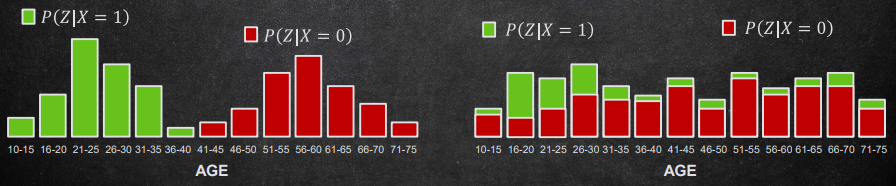
\includegraphics[width=\textwidth]{img/overlap.png}
    \caption{Example of overlap}
    \label{fig:positivity}
\end{figure}

Adjusting on a lot of covariets can lead to \textbf{curse of dimensionality}, because
all the subgrup can be contained in the control group or in the treatment group.

Another important assumption is the \textbf{no interference} assumption.
\begin{definition}[No interference]
    The outcome $Y_i$ of the $i^{th}$ individual is not affected by anyone else's
    treatment $X_j$ for $j \neq i$.
    \begin{equation}
        Y_i(x_1, x_2, \ldots, x_i, \ldots, x_n) = Y_i(x_i)
    \end{equation}
\end{definition}

The last assumption is the \textbf{consistency} assumption.
\begin{definition}[Consistency]
    If the treatment is $X$, then the observed outcome $Y$ is the potential outcome
    under treatment $X$. Formally:
    \begin{equation}
        X = x \rightarrow Y = Y(X)
    \end{equation}
\end{definition}

We need the treatment to be well defined, if consistency is not respected $Y(1)$
is not well defined since it will be $1$ or $0$ and it depends on something that
is not captured  by the treatment $X$.

\begin{definition}[Stable Unit Treatment Value Assumption]
    The \textbf{Stable Unit Treatment Value Assumption} (SUTVA) is satisfied if
    individual $i$'s outcome $Y_i$ is simply a function of the treatment $X_i$.
\end{definition}

SUTVA is a combination of consistency, no interference and deterministic potential
outcome.

Now, we need to introduce some terminology that will be useful in the following
chapters.
\begin{itemize}
    \item \textbf{Estimand}: The quantity that we want to estimate.
    \item \textbf{Estimate}: an approximation of the estimand, which we get
          using data.
    \item \textbf{Estimator}: a function that maps the data to an estimate of the
          estimand.
    \item \textbf{Estimation}: the process that we use to go from data plus the
          estimand to a concrete number is known as estimation.
    \item \textbf{Causal estimand}: refers to any estimand that contains a potential
          outcome in it.
    \item \textbf{Statistical estimand}: refers to any estimand that does not contain
          a potential outcome in it.
\end{itemize}

The process of estimation is shown in figure \ref{fig:pipeline}. We need to
introduce also the concept of \textbf{identification}, which is the process of
moving a causal estimand to an equivalent statistical estimand. And the concept
of \textbf{Estimation}, which is the process of moving from a statistical estimand
to an estimate.
\begin{figure}[!ht]
    \centering
    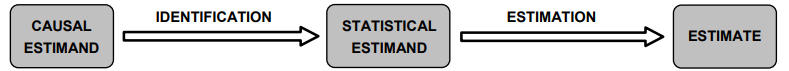
\includegraphics[width=\textwidth]{img/process.png}
    \caption{Process of estimation}
    \label{fig:pipeline}
\end{figure}

When we want to answer to causal estimand, so a question thet we want to answer when
we do something so we interactive, we want to pass to a statistical estimand
to prove our answer using observation datas and this process of passing from causal
estimand to statistical estimand is called identification. Not always is possible
to do identification. When exist identification, we can answer an intervational query
without intervening on the experiment.

To do identification we need a causal model, so we define some assumption on causal
relationship between variables and this define if a causal estimand could be translate
in a statistical estimand.

Generaly in AI everyone wants to take decision using observation estimand computed
on data, but these are all subjected to bias.
\chapter{Flow of Association}
Assume we only care about modeling association, without any causal modeling. If
we want to model the data distribution $P(X_1, X_2, \ldots, X_n)$, we can use
the chain rule of probability to decompose it into a product of conditional
distributions:
\begin{equation}
    P(X_1, X_2, \ldots, X_n) = P(X_1)P(X_2|X_1)P(X_3|X_1, X_2)\ldots P(X_n|X_1, X_2, \ldots, X_{n-1})
\end{equation}
However, if we were to model discrete random variables by using probability
tables, it would take an exponential number of parameters. To solve this we
can model local dependencies between variables to reduce the number of
parameters.

\begin{definition}[\textbf{Local Markov Assumption}]
    Given all the parents $pa(x)$ of a node $x$ in a DAG, the local Markov
    assumption states that $x$ is independent of all its non-descendants.
\end{definition}
Talking about Bayesian networks, the local Markov assumption is equivalent to
the \textbf{bayesian network factorization}:
\begin{equation}
    P(X_1, X_2, \ldots, X_n) = \prod_{i=1}^n P(X_i|pa(X_i))
\end{equation}

At this point we can define a \textbf{markov probability distribution} as a
probability distribution $P$ that satisfies the local Markov assumption with
respect to a DAG $G$.

As important as the local Markov assumption is, it only gives us information
about the independencies in $P$ that a DAG $G$ implies.

To get this guaranteed dependence between adjacent nodes, we will generally
assume a slightly stronger assumption than the local Markov assumption, called
the \textbf{minimality assumption}.
\begin{definition}[\textbf{Minimality Assumption}]
    The minimality assumption means:
    \begin{enumerate}
        \item \textbf{local markov assumption}: Given all the parents $pa(x)$ of
              a node $x$ in a DAG, the local Markov assumption states that $x$
              is independent of all its non-descendants.
        \item Adjacent nodes in the DAG $G$ are dependent.
    \end{enumerate}
\end{definition}

Because removing edges in a Bayesian network is equivalent to adding
independencies, the minimality assumption is equivalent to saying that we can't
remove any more edges from the graph $G$.

\begin{definition}
    $P$ and $G$ are Markov Compatible if $P$ factorize according to $G$. 
\end{definition}

Up to now all we presented was about statistical models and modeling association.
We now need to introduce some causal assumptions, turn them into causal models
for allowing the study of causation. In order to introduce causal assumptions,
we must first understand what it means for $X$ to be a cause of $Y$. We can simply
define \textbf{cause} as follows:
\begin{definition}[\textbf{Cause}]
    $X$ is a cause of $Y$ if changing $X$ changes $Y$.
\end{definition}

Also, we can define \textbf{(strict) causal edges assumption} in a DAG $G$ as every parent
is a direct cause of all its children. Given this assumption, we can define a
\textbf{Causal graph} as a DAG $G$ that satisfies the causal edges assumption.

Adding the causal edges assumption, implies that directed paths in the DAG take
on a very special meaning; they correspond to \textbf{causation}. This is in
contrast to other paths in the graph, which association may flow along, but
causation certainly may not.
\section{Basic Structure}
To understand the difference between association flow and causal flow in DAGs,
we need the following minimal building blocks
\begin{itemize}
    \item chain
    \item fork
    \item collider
    \item two un-connected nodes
    \item two connected nodes
\end{itemize}
\begin{figure}[!ht]
    \centering
    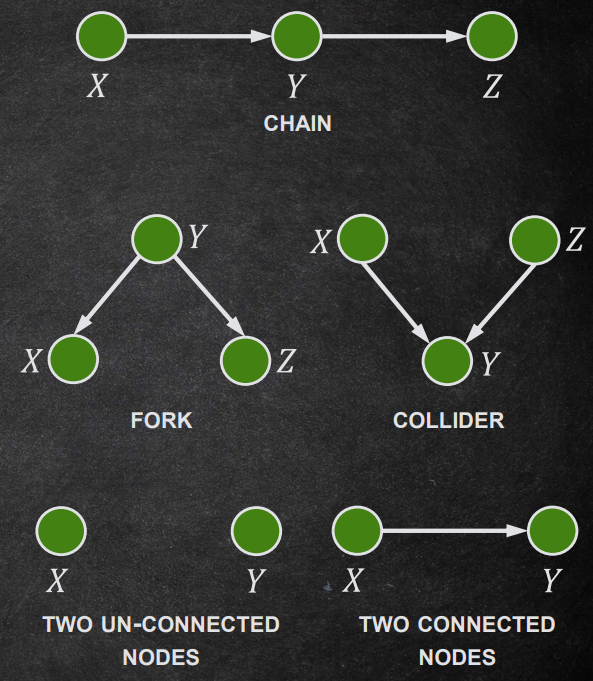
\includegraphics[width=0.7\textwidth]{img/basic_bn.png}
    \caption{Basic elements of a DAG}
\end{figure}

By flow of association, we mean whether any two nodes in a graph are associated
or not associated. In other terms, we want to know whether two nodes are
(statistically) dependent or (statistically) independent. However, we will also
study whether two nodes are conditionally independent or not.
\subsection{Two un-connected nodes}
Given a graph consisting of just two unconnected nodes, these nodes are not
associated, because there is no edge between them. To show this, consider the
factorization of the joint probability $P(X, Y)$ that the Bayesian network
factorization gives us: $P(X, Y) = P(X)P(Y)$. This factorization immediately
gives us a proof that the two nodes are unassociated (independent).
\subsection{Two connected nodes}
On the contrary, if there is an edge between the two nodes, then the two nodes
are associated. We exploit the causal edges assumption which means that $X$ is
a direct cause of $Y$. They are dependent and conditional dipendent.
\subsection{Chain and Fork}
We can consider this two building blocks together, because they share the same
set of dependencies. In both cases, the association flows from $X$ to $Z$ through
$Y$.

They also share the same set of independencies. When we condition on $Y$ in both
graphs, it blocks the flow of association from $X$ to $Y$. Therefore, when we
condition on $Y$ ( $Z$'s parent in both graphs), $Z$ becomes independent of (and
viceversa). This independence is an instance of a \textbf{blocked path}.
\begin{note}
    The flow of association in general is symmetric, but the flow of causation
    is not.
\end{note}
\subsection{Collider}
Association flows along any path that does not contain a \textbf{collider}. A
collider is a node with two or more parents that are independent $X \perp Z$.
We can think of $X$ and $Z$ simply as unrelated events that can happen, and which
both contribute to some common effect ($Y$). To show that $X \perp Z$ we apply
the Bayesian network factorization and then marginalize out $Y$.

The collider $Y$ blocks the path from node $X$ to node $Z$ and blocks the path
from node $Z$ to node $X$. This is another example of a blocked path, but this
time the path is not blocked by conditioning; the path is un-blocked by conditioning
on a collider.

Conditioning on descendants of a collider also induces association in between the
parents of the collider. The intuition is that if we learn something about a
collider's descendant, we usually also learn something about the collider itself
because there is a direct causal path from the collider to its descendants, and
we know that nodes in a chain are usually associated assuming minimality.
\section{D-separation}
\begin{definition}[\textbf{D-separation}]
    A path $p$ is blocked by a set of nodes $S$ if and only if:
    \begin{itemize}
        \item $p$ contains a chain of nodes or a fork such that the middle node
              is in $S$.
        \item $p$ contains a collider such that the collision node is not in $S$,
              and no descendant of the collision node is in $S$.
    \end{itemize}
    If $S$ blocks \textbf{every} path between two nodes $X$ and $Y$, then $X$ and
    $Y$ are \textbf{d-separated}, conditional on $S$, and thus are independent
    conditional on $S$.
\end{definition}
D-separation is an extremely important concept, because it implies conditional
independence. This is a very powerful tool for reasoning about causal models.
\begin{itemize}
    \item $X \perp_G Y | S$ implies that $X$ and $Y$ are d-separated in the DAG
          $G$ when conditioning on $S$.
    \item $X \perp_P Y | S$ implies that $X$ and $Y$ are independent in the
          distribution $P$ when conditioning on $S$.
\end{itemize}
\begin{definition}[\textbf{Global Markov Assumption}]
    Given that $P$ is Markov with respect to a DAG $G$, if $X$ and $Y$ are d-separated
    in $G$ conditional on $S$, then $X$ and $Y$ are independent conditional on $S$.
\end{definition}

Not only is association not causation, but causation is a sub-category of
association, thus association and causation both flow along directed paths.

We can tell if two nodes are not associated by whether or not they are d-separated.

If we want to measure the causal effect of $X$ on $Y$, we need to ensure that $X$
and $Y$ are d-separated in the augmented graph where we remove outgoing edges
from $X$. This is the only way to ensure that the association we measure is causation.

\begin{note}
    Association is symmetric while causation not.
\end{note}

To summerizing every assumptions:
\begin{itemize}
    \item local/global Markov Assumption: tells us which nodes are unassociated, tells 
    along which paths the association doesn't flow
    \item Minimality assumption: tells us which paths association does flow along
    \item Causal edges assumption: tells us causation flows along directed paths.
\end{itemize}
\begin{figure*}[!h]
    \centering
    \includegraphics*[width=\textwidth]{img/causal_networks_assumptions.png}
\end{figure*}


\chapter{Causal Models}
\section{The do-operator and Interventional Distributions}
As you have undoubtedly heard many times in statistics classes, “correlation is
not causation.” A mere association between two variables does not necessarily
mean that one of those variables causes the other. For this reason, the
\textbf{randomized controlled experiment} is considered the standard of statistics.

We can define a randomized controlled experiment as an experiment in which all
the \textbf{factors} that influence the outcome of the experiment are either
static, or vary at random, except for one. This implies that any change in the
outcome variable must be due to that one input variable, so we can control a factor
and study how the outcome changes. This type of experiments allows us to find causal
relationships, so we can answer to causal queries.

In cases where randomized controlled experiments are not practical, researchers
instead perform \textbf{observational studies}, in which they merely record data,
rather than controlling it. In these cases, the problem is that is difficult to
untangle the effects of different variables.

We can summarize the difference between these two types of studies as follows:
\begin{itemize}
      \item \textbf{Intervening}: we change the system assigning values to the a
            variable and observing the effect on the other variables. When we
            intervene to fix the value of a variable, we curtail the natural
            tendency of that variable to vary in response to other variables in
            nature. This amounts to performing a surgery on the graphical model,
            which we do by removing all edges directed into that variable.
            Intervening would be to take the whole population and give everyone
            treatment. This is possible if we can control the experiment, because
            we can apply a treatment to the entire population.
      \item \textbf{Conditioning}: we merely narrow our focus to the subset of
            cases in which the variable takes the value we are interested in.
            So, conditioning on $X = x$ just means that we are restricting our
            focus to the subset of the population to those who received treatment.
\end{itemize}
We denote intervention with the \textbf{do-operator} $do(X=x)$. So, if we have
an expression which contains the do-operator, we know that we are intervening
on that variable and we call this expression a \textbf{interventional expression}.
When do do-operator doesn't appear in the expression so the expression is called
\textbf{observational}.

An \textbf{interventional expression} which can be reduced to an \textbf{observational expression}
is said to be \textbf{identifiable}. This means that we can estimate the effect
of the intervention from the observational data.

An \textbf{estimand} is said to be:
\begin{itemize}
      \item \textbf{causal}: it contains the do-operator
      \item \textbf{statistical}: it doesn't contain the do-operator
\end{itemize}

Whenever, $do(x)$ appears in expression after the conditioning bar, it means
that everything in that expression is in the \textbf{post-intervention world}
where intervention $do(x)$ occurs.


\section{Modularity and Adjustment Formula}
We can define a \textbf{causal mechanism} as a mechanism that generates $X_i$ as
the conditional distribution of $X_i$ given its parents (causes) $pa(X_i)$.

Also, we want to show that intervention are local. This means that intervening on
a variable $X_i$ only changes the causal mechanism for $X_i$; it does not change
the causal mechanisms that generate any other variables $X_j$.
\begin{definition}[\textbf{Modularity - indipendent mechanism - invariance of Causal Models}]
      If we intervene on a set of nodes $S$, setting them to constants, then for
      all $X_i \in \{X_1, \ldots, X_n\}$ we have the following:
      \begin{itemize}
            \item If $X_i \notin S$ then the causal mechanism that generates $X_i$
                  is unchanged by the intervention.
            \item If $X_i \in S$ then the causal mechanism that generates $X_i$ is
                  replaced by a constant. In other words, $P(X_i | pa(X_i)) = 1$
                  if $x$ is the value that $X_i$ is set to by the intervention
                  $do(X_i = x)$. Otherwise, we have $P(X_i | pa(X_i)) = 0$.
      \end{itemize}
\end{definition}
\begin{note}
      The \textbf{causal graph} for \textbf{interventional (experimental) distributions} is simply
      the same graph that was used for the observational joint distribution, but
      with all of the edges to the intervened node(s) removed.
\end{note}
Using do-expressions and graph surgery, we can begin to untangle the causal
relationships from the purely associative.


Not always modularity is statisfied, for example when we apply $do(X_1=x)$
and at the same time $P(X_4=x|X_3)$ changes, in this example modularity wasn't
fulfilled. In the reality this happens when we have hidden factor, so we
should investigate on this factor to remove it.

\begin{note}
      It is worth noting here that we are making a tacit assumption that
      the \textbf{intervention} has no side effects. This means that applying intervention
      this never change values for other variables.
\end{note}

The intervention procedure, which led to the \textbf{Adjustment Formula},
dictates that $Z$ should coincide with the parents $pa(X)$ of $X$, because it is
the influence of these parents that we neutralize when we fix $X$ by external
manipulation $do(X)$, so we are blocking the association path between X and Y througth
Z, setting Z.

We can therefore write a general Adjustment Formula on a set of variables and summarize it in a rule:
\begin{definition}[\textbf{Causal effect rule}]
      Given a graph $G$ in which a set of variables $pa(X)$ are designed as the
      parents of a set of variables $X$, the \textbf{causal effect} of $X$ on $Y$ can be computed
      as follows:
      \begin{equation}
            P(Y = y| do(X = x)) = \sum_{u} P(Y | X = x, pa(X) = u)P(pa(X) = u)
      \end{equation}
      where $u$ ranges over all the combinations of values that the variables in
      $pa(X)$ can take, so we are adjusting for Z or controlling for Z.
\end{definition}

So we will start from \textbf{causal estimand} $P(Y=y|do(X=x))$ and for the causal effect
rule we arrive to the \textbf{statistical estimand} which is  $\sum_z P(Y=y|X=x, Z=z) P(Z=z)$ after
the inverversion on X. This is possible if and only if modularity is satisfied.

If we apply some manipulation on the formula, we can obtain a more convenient
form that is equivalent beacause we are moltiplying and dividing by the same quantity:
\begin{equation}
      P(Y = y| do(X = x)) = \frac{\sum_{u} P(Y = y, X = x, pa(X) = u)P(pa(X) = u)}{P(X = x | pa(X) = u)}
\end{equation}
In the equation above, the denominator $P(X = x | pa(X) = u)$ represents the \textbf{propensity score}
which displays the role played by the parents $pa(X)$ of $X$ in determining the
result of the intervention $do(X = x)$.

\section{Truncated Factorization and Backdoor Adjustment}
In some circumstances, we can involve multiple interventions in the same time.

The previous consideration also allows us to generalize the Adjustment Formula to
\textbf{multiple intervansions}, that is, interventions that fix the values of a
set of variables $S$ to constants $s$. We simply write down the Factorization of
the pre-intervention distribution and strike out all factors that correspond to
variables in the intervention set $S$.

\begin{definition}[\textbf{Truncated Factorization (G-formula)}]
      We assume that $P$ and $G$ satisfy the Markov assumption and modularity.
      Given, a set of intervention nodes $S$, if $x_i$ is consistent with the
      intervention $S = s$, then:
      \begin{equation}
            P(x_1, x_2, \dots, x_n| do(S = s)) = \prod_{X_i\not \in S}^{n} P(X_i = x_i | pa(X_i))
      \end{equation}
      otherwise $P(x_1, x_2, \dots, x_n| do(S = s)) = 0$.
\end{definition}

\begin{note}
      Remember that pre-intervention distribution of a graph G is defined by the
      Bayesian Network Factorization as follow:
      $$P(X_1 = x_1, X_2=x_2, \dots, X_n=x_n) = \prod_{i=1}^{n} P(X_i=x_i | pa(X_i))$$
      While the post-intervention distribution of a graph G with an intervention of
      $S=s$ is defined as followed:
      $$P(X_1 = x_1, X_2=x_2, \dots, X_n=x_n | do(S=s)) = \prod_{X_i\not \in S}^{n} P(X_i=x_i | pa(X_i))$$
      And there is a relationship between them that is defined by:
      $$P(X_1 = x_1, X_2=x_2, \dots, X_n=x_n | do(S=s)) = \frac{P(X_1 = x_1, X_2=x_2, \dots, X_n=x_n)}{P(S=s | pa(S))}$$
      And $P(S=s | pa(S))$ is the \textbf{propensity score}.
\end{note}

Not always in every condition we can use the \textbf{causal effect rule}, infact,
in the graph represented below we have \textbf{unmeasured parents} that impact on
$X$ and $Y$, also known as
\textbf{latent}, that, though represented in the graph, may be inaccessible for
measurement. In those case, we can't adjust on each values of $pa(X)$ because we
can't measure so we need to find an alternative set of variables to adjust for.

\begin{figure}[h]
      \centering
      \includegraphics*[width=0.7\textwidth]{img/unmeasured_parents.png}
\end{figure}

\begin{center}
      Under what conditions, is the structure of the causal graph sufficient for
      computing a causal effect from a given data set?
\end{center}

We have decided to represent causal stories with graphs so the solution becomes a graph theretical
solution.

One of the most important tools we use to determine whether we can compute a
causal effect is a simple test called the \textbf{backdoor criterion}. Using it,
we can determine, for any two variables $X$ and $Y$ in a causal model represented
by a DAG $G$, which set of variables $S$ in that model should be conditioned on
when searching for the causal relationship between $X$ and $Y$.

\begin{definition}[\textbf{Backdoor criterion}]
      Given an ordered pair of variables $(X, Y)$ in a DAG $G$, a set of variables
      $S$ satisfies the backdoor criterion relative to $(X, Y)$ if no nodes
      in $S$ are descendants of $X$ and $S$ blocks all backdoor paths between $X$
      and $Y$ that contain an arrow into $X$.

\end{definition}
\begin{definition}[\textbf{Backdoor paths}]
      A Backdoor path is a path from $X$ to $Y$ is when there is an entering arrow in $X$.
\end{definition}

\begin{definition}[\textbf{Backdoor adjustment}]

      If a set of variables $S$ satisfies the backdoor criterion relative for $X$ and
      $Y$, and positivity, then the causal effect of $X$ on $Y$ is given by the following new version
      of adjusted formula:
      \begin{equation}
            P(Y = y| do(X = x)) = \sum_{s} P(Y = y| X = x, S = s)P(S = s)
      \end{equation}
      just as when we adjust for the parents of $X$ in the Adjustment Formula.
\end{definition}


\begin{note}
      $pa(X)$ satisfied backdoor criterion.
\end{note}

In general, we would like to condition on a set of nodes $S$ such that we:
\begin{itemize}
      \item Block all the spurious paths between $X$ and $Y$. We want the
            conditioning set $S$ to block any \textbf{backdoor path} in which
            one end has an arrow into $X$, because such paths may make $X$ and
            $Y$ dependent. (confounding effect)
      \item Leave all directed paths from $X$ to $Y$ unchanged. We don't want
            to condition on any nodes that are descendants of $X$.
      \item Create no spurious paths
\end{itemize}
\begin{figure}[!ht]
      \centering
      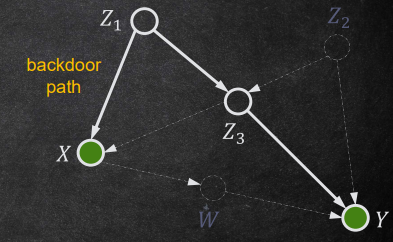
\includegraphics[width=\textwidth]{img/backdoor.png}
      \caption{Backdoor paths}
      \label{fig:backdoor}
\end{figure}
\begin{definition}[\textbf{Backdoor Adjustment Formula}]
      Give the modularity assumption, that, $S$ satisfies the backdoor criterion,
      and positivity, we can identify the causal effect of $X$ on $Y$ as follows:
      \begin{equation}
            P(Y = y| do(X = x)) = \sum_{s} P(Y = y| X = x, S = s)P(S = s)
      \end{equation}
\end{definition}

We can use the backdoor adjustment formula if, $S$ d-separates $X$ from $Y$ in
the augmented graph obtained by removing all outgoing edges from $X$.

We would be able to isolate the causal association if $X$ is d-separated from
$Y$ in the augmented graph.
\begin{center}
      \textbf{Isolation of the causal association is identification}
\end{center}

We can also isolate the causal association if $X$ is d-separated from $Y$ in
the augmented graph, conditional on $S$. This is what the first part of the
backdoor criterion is about and what we've codified in the backdoor adjustment.
\chapter{Structural Causal Model}
Graphical causal models such as causal bayesian network give us powerful ways to encode 
statistical and causal assumptions, but we have yet to explain exactly what an intervantion
is or exactly what a causal mechanism is.

Moving from causal Bayesian networks to \textbf{full Structural causal models} will give 
us this additional clarity along with the power to compute \textbf{counterdactuals}.

We need a way to specify the following concept:
\begin{center}
    A causes B
\end{center}

this means that changing A changing also B but changing B doesn't mean changing A.

we can use the following notation $B := f(A)$ and can be read as we assign to B the 
value $f(A)$ and this ($:=$) is asimmetric different by using $=$.  

\begin{note}
    Using $B := f(A)$ we are using a \textbf{causal model}, while $B = f(A)$ we 
    are using a \textbf{statistical model}
\end{note}

This operetor ($:=$) is deterministic. Ideally, we'd like to allow it to be 
probabilistic, which allows room for some unknown causes ($U$) of $B$ that factor into 
this mapping. Then, we write the \textbf{structural equation} as:
\begin{equation}
    B := f(A, U)
\end{equation}
This means that the function $f$ is deterministic (is a stochastic mapping) applied on
$A$ that we know with some noise $U$ that models the unknown causes.

\begin{figure}[h]
    \centering
    \includegraphics*[width=0.7 \textwidth]{img/uknown_graphs.png}
\end{figure}

When isnot specified we are in the \textbf{nonparametric regime} because we aren't making 
any assumptions about parametric form. However, \textit{structural equations} can 
represent any stochastic mapping, so generalize the \textit{probabilistic factor}:
\begin{equation}
    P(X_i|pa(X_i))
\end{equation}

Therefore, all the results that we've seen such as the and the truncated factorization and the 
backdoor adjustment still hold when we introduce structural equations.

We have now come to the more precise definitions of what a cause is and what a causal
mechanism is.

\begin{definition}
    A causal mechanism that generates a variable is the structural equation 
    that corresponds to that variable.
\end{definition}

\begin{note}
    Cause is more general than directed cause.
\end{note}

From the initial model $B:=f(A,U)$ the $A,U$ are directed cause for $B$.


In general, a model can consist of more than one structural equation, for example:
\begin{equation}
    M : \begin{array}{l}
        B := f_B(A, U_B) \\ C := f_C(A, B, U_c) \\ D := f_D(A, C, U_D)
    \end{array}
\end{equation}

The associate causal graph is

\begin{figure}[h]
    \centering
    \includegraphics*[width=0.5 \textwidth]{img/graph_associate_structural_equation.png}
\end{figure}

Based on the previous example, we can distinguish $A, U_B, U_C, U_D$ as \textbf{
    exogenous variables}, i.e., they can not be descendant of any other variables, 
and in particular, they can not be descendant of an endogenous variable; they have 
no ancestors and are represented as root nodes in graphs.

\begin{definition}[\textbf{exogenous variables}]
    The exogenous variables are the variables for wich we don't have a structural equation
    that explains their behavior, so they are root node in the graph.
\end{definition}

They are external to the model; we chose, for whatever reason, not to explain how 
they are caused (we don't care about cause of cause).

While, $B, C, D$ are \textbf{endogenous variables}, i.e., the variables that we write 
structural equations for, i.e., the variables whose causal mechanisms we are modeling.
 
\begin{definition}[\textbf{endogenous variables}]
    The endogenous variables are the variables for wich we have a structural equations
    that define their behavior, so they have parents in the graph.
\end{definition}

If we know the value of every \textbf{exogenous variable}, then using the functions of the 
structural equations, we can determine with perfect certainty the value of every
\textbf{endogenous variable}.

\begin{definition}[\textbf{structural causal model}]
    A structural causal model is a tuple $M = \langle U, V, F \rangle$ of the following
    sets:
    \begin{itemize}
        \item $U$ is a set of exogenous variables.
        \item $V$ is a set of endogenous variables.
        \item $F$ is a set of functions, one to generate each endogenous variable as a 
        function of other variables.
    \end{itemize}
\end{definition}

Every structural causal model implies an associated \textbf{causal graph}: for each 
structural equation, draw an edge from every variable on the right-hand side to the 
variable on the left-hand side.

If we have a causal graph contains no cycles (it is a DAG) and the \textbf{noise variable} 
are:
\begin{itemize}
    \item \textbf{indipendet} so the causal model is \textbf{markovian}
    \item \textbf{dipendet} so the causal model is \textbf{semi-markovian}
\end{itemize} 

\begin{note}
If there is a \textbf{unobserved confounding} the model is \textbf{semi-markovian}. And 
the graph of non-markovian models contains cycles.
\end{note}

\textbf{Intervantion} in SCMs consist of replacing the structural equation, i.e., if the 
intervention is $do(X = x)$ then we replace the structural equation associated with $X$.
For example:
\begin{equation}
    M : \begin{array}{l}
        Z := U_Z \\ X := f_X(Z, U_X) \\ Y:= f_Y(X, Z, U_Y)
    \end{array}
\end{equation}
The graph assosiated is Markovian. If we do the following intervension as $do(X=x)$
so the structural equation will be:
\begin{equation}
    M_X : \begin{array}{l}
        Z := U_Z \\ X := x \\ Y:= f_Y(X, Z, U_Y)
    \end{array}
\end{equation}
and the graph will be modified removing the edge between $U_X$ and $X$. Below you 
can see how the graph change.


\begin{figure}[h]
    \centering
    \includegraphics*[width=0.5 \textwidth]{img/intervention_on_structural_eq.png}
\end{figure}

Only changes the equation for $X$ and no other variables is a consequence of the \textbf{modularity
assumption}; these causal mechanisms are modular.

\begin{definition}[\textbf{Modularity assumption for SCM}]
    Consider an SCM $M=\langle U, V, F \rangle$ and an interventional SCM $M_x =\langle U, V, F_x \rangle$,
    that we get by performing the intervantion $do(X = x)$. The modularity assumption states 
    that $M$ and $M_x$ share all of their structural equations except the structural equation
    for $X$, which is $X := x$ in $M_x$. 
\end{definition}

For the modularity the intervention $do(X=x)$ is localized to $X$.

We can write unit level potential outcome as:
\begin{itemize}
    \item $Y_x (u)$ potential outcome that unit $u$ would observe if taking treatment
        $X = x$, given that the SCM is $M$.
    \item $Y_{M_x}(u)$ potential outcome that unit $u$ would observe if taking treatment
        $X = x$, given that the SCM is $M_x$ (in the manipulated model).
\end{itemize}

The \textbf{law of counterfactuals} gives us information about counterfactuals:
\begin{equation}
    Y_x(u) = Y_{M_x}(u)
\end{equation}

Given an SCM with enough details about it specified, we can actually compute 
counterfactuals. This is extremely important because it is exactly what the fundamental 
problem of causal inference told us we cannot do.

Not only did we specify that the adjustment set blocks all backdoor paths from $X$ to $Y$,
but we also specified that does not contain any descendants of $X$, otherwise we have 
a selection bias effect. 

There are two categories of things that could go wrong if we condition on descendants 
of $X$:
\begin{enumerate}
    \item We block the flow of causation from $X$ to $Y$. 
    \item We induce non-causal association between $X$ and $Y$, we generate a spurius 
    path not existed before.
\end{enumerate}

In the first case, if we have a chain between $X$ and $Y$ and we have at least a 
node $L$ that is a mediator of the causal effect of $X$ on $Y$. So when 
we observe $L$ we mesure a $0$ causal effect between $X$ and $Y$ because it's blocked 
by the observation on the mediator. If we have a mediator with an observation and direct link from $X$ 
to $Y$ so we can measure the direct cause effect of $X$ on $Y$ but not the undirect.

In the second case, if we have a direct link between $X$ and $Y$ and a collider 
on $L$ that is a discendant of $X$ and $Y$, if we condition on a descendant of $L$ 
that isn't a mediator, it could unblock a path 
from $X$ to $Y$ that was blocked by a collider, so we are introducing a \textbf{collider bias}. 
The same holds true for any descendant of $L$. So we should only control the counterfactuals.

It is worthwhile to notice that we actually can condition on some descendants of $X$ 
without inducing non-causal associations between $X$ and $Y$.
Conditioning on descendants of $X$ that aren't on any causal paths from $X$ and $Y$
won't induce bias.

Even outside of graphical causal models, this rule is often applied; it is usually described 
as not conditioning on any \textbf{post treatment variables}.

Unfortunately, even if we only condition on \textbf{pre treatment covariates}, we can still 
induce \textbf{collider bias} if we condition on the collider.
Doing this opens up a backdoor path, along which non-causal association can flow. This is 
known as $M$-Bias due to the $M$-Shape that this non-causal association flows along 
when the graph is drawn with children below their parents.

\section{Application of Backdoor Adjustment}
In this section we will show how to derive the \textbf{associational} quantity 
$\mathbb{E}[Y|X = x]$ (it is the observational value obtained without interversion),
 that will be compared to the \textbf{causal} quantity $\mathbb{E}[Y|do(x)]$. There 
 are situations where the causal quantity is the same to the associational.

If the treatment were binary, then we would just look at the difference between 
the quantities with the respected value. However, if we consider \textbf{linear 
generative process}, thus quantities are:
\begin{equation}
    \frac{\partial\mathbb{E}[Y |x]}{\partial x } \, \land \, \frac{\partial\mathbb{E}[Y |do(x)]}{\partial x}
\end{equation}
this formulation give us all the information about the treatment effect, regardless of if treatment is continuous, binary, or multi-valued.

\begin{note}
    In this section we will assume \textbf{infinite} data so we can work with expectations. 
    It's a strong absumption but helps in explain the situation. 
\end{note}

For the rest of this section we will consider the example given in figure ref{fig:example}. This can also be represented as follows:
\begin{equation}
    \begin{array}{l}
         X := \alpha_1 Z \\ Y := \beta X + \alpha_2 Z 
    \end{array}
\end{equation}
where $\beta$ is the causal effect of X on Y and $\alpha_1, \alpha_2, \beta\in \mathbb{R}$.

\begin{figure}[!ht]
    \centering
    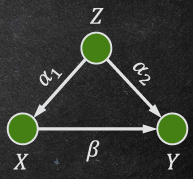
\includegraphics[width=0.2\textwidth]{img/example.png}
    \caption{Basic example}
    \label{fig:example}
\end{figure}

Let’s now prove that $ beta$ is the causal effect of $X$ on $Y$. Given the ordered 
pair $(X, Y)$ and the set $S  = \{Z \}$ which represents the \textbf{sufficient 
adjustment set} we have the following:
\begin{equation} 
    \begin{array}{ll}
         \mathbb{E}[Y | do(x)] = \mathbb{E}_Z[\mathbb{E}[Y | X = x, Z]] & = \mathbb{E}_Z[\mathbb{E}[\beta X + \alpha_2 Z | X = x, Z]] \\
         & = \mathbb{E}_Z[\mathbb{E}[\beta x + \alpha_2 Z]]\\
         & = \mathbb{E}_Z[\beta x + \alpha_2 Z] \\
         & = \beta x + \alpha_2\mathbb{E}[Z]
    \end{array}
\end{equation}
then, we have the following:
\begin{equation}
    \frac{\partial \mathbb{E}[Y |do(x)]}{\partial x} = \frac{\partial [\beta x + \alpha_2\mathbb{E}[Z]]}{\partial x} = \beta
\end{equation}

While, when we are talking about \textbf{associational effect} from $X$ to $Y$ we have:
\begin{equation} 
    \begin{array}{ll}
         \mathbb{E}[Y | x] = \mathbb{E}[Y | X = x] & = \mathbb{E}[\beta X + \alpha_2 Z | X = x] \\
         & = \beta x + \mathbb{E}[\alpha_2 Z |X = x]\\
         & = \beta x + \alpha_2 \mathbb{E}[Z |X = x] \\
         & = \beta x + \frac{\alpha_2}{\alpha_1} x
    \end{array}
\end{equation}
then, we have the following:
\begin{equation}
    \frac{\partial \mathbb{E}[Y |x]}{\partial x} = \frac{\partial[\beta x + \alpha_2 \mathbb{E}[Z |X = x]]}{\partial x} = \beta + \frac{\alpha_2}{\alpha_1}
\end{equation}
Therefore, it is clear that \textbf{associational effect} of  $X$ on $Y$ is different from the \textbf{causal effect} of $X$ on $Y$.

In the potential outcomes framework, it is common to only condition on pretreatment 
covariates. This would prevent a practitioner who adheres to this rule from conditioning on the collider. However, there is no reason that there can’t be pre treatment colliders that induce $M$ bias.

Given, the two assumptions: \textbf{modularity assumption} and \textbf{markov assumption}
and \textbf{positivity}, if the backdoor criterion is satisfied in our assumed causal graph, 
then we achieve \textbf{identification}.

\begin{note}
    Note that although the a backdoor criterion is a sufficent condition for identification, it is not a necessary condition.
\end{note}
\begin{note}
    No interference assumption in commonly implicit in causal graph because the $Y$
    usually only has a single node $X$ for treatment as a parent. In other way 
    consistency follows from the axioms of SCMS. Contrary the positivity is still important 
    assumption that we must make.    
\end{note}


\chapter{Randomized Experiments}
\textbf{Randomized experiments} are noticeably different from observational studies.
In randomized experiments, the experimenter has complete control over the treatment
assignment mechanism.

This complete control over how treatment is chosen is what distinguishes randomized experiments from observational studies. In this simple experimental setup, the treatment 
isn’t a function of covariates at all. In observational studies, the treatment is almost always a function of some of the covariate(s).

This difference is key to whether or not confounding is present in our data.

In randomized experiments, \textit{association} = \textit{causation} because they guarantee that there is no confounding.
\begin{equation}
    \mathbb{E}[Y(1)] -  \mathbb{E}[Y(0)] = \mathbb{E}[Y| X = 1] - \mathbb{E}[Y | X = 0]
\end{equation}

Since the treatment and control groups would be the same, in all aspects, except for treatment $X$, any difference in the outcomes $Y$ of the treatment and control groups is due to the treatment $X$.
\begin{definition}[\textbf{Covariate balance}]
    We have \textbf{covariate balance} if the distribution of covaraiates $Z$ is the same across treatment groups.
    \begin{equation}
        P(Z|X = 1) = P(Z|X = 0)
    \end{equation}
\end{definition}

Randomization implies covariate balance, across all covariates $Z$, even unobserved ones. Intuitively, this is because the treatment is chosen at random, regardless of $Z$, so the treatment and control groups should look very similar. 

We will now prove that association is equal to causation in randomized experiments by proving that:
\begin{equation*}
    P(Y|do(x)) = P(Y|x)
\end{equation*}
For the proof, the main property we utilize is that covariate balance implies $Z$ and $X$ are independent.

First, let $S = Z$ be a \textbf{sufficent adjustment set} that potentially contains unobserved variables. Such an \textbf{adjustment set} $S$ must exist because we allow it to contain any variables, observed or unobserved. 

Then, from the backdoor adjustements we get:
\begin{equation}
    \begin{array}{ll}
        P(y|do(x)) & = \sum_s P(y|x, S = s)P(S = s)  \\
            & = \sum_s \frac{P(y|x, s)P(x|s)P(s)}{P(x | s)} \\
            & = \sum_s \frac{P(y, x, s)}{P(x | s)} \\
            & = \sum_s P(y, s| x) \\
            & = P(y | x)
    \end{array}
\end{equation}

\textbf{Exchangeability} gives us another perspective on why randomization makes causation equal to association. If the groups are exchangeable, we could exchange these groups, and the average outcomes would remain the same.

The final perspective that we'll look at to see why association is causation in randomized experiments is that of \textbf{graphical causal models}.

In regular observational data, there is almost always confounding. However, if we randomize  it doesn't depend on anything other than the output of a coin toss. Since the node has no incoming edges and thus no backdoor paths exist.
\chapter{Non-parametric Identification}
\section{Frontdoor Adjustment}
We have seen that the \textbf{backdoor criterion} is sufficient for identification
but not necessary. In other words, is it possible to get identifiability without
being able to block all backdoor paths? Also, if we have unobserved variables we
\textbf{cannot} block the backdoor path.

If we are only focusing on the data we can have multiple interpretations of them.
So we need a method that we can use for causal estimation.

This can be obtained by chaining together the partial effects to obtain the overall effect.
\begin{definition}[\textbf{Frontdoor Criterion}]
    A set of variables $\mathbf{S}$ is said to satisfy the front-door criterion
    relative to an ordered pair of variables $(X, Y)$ if:
    \begin{enumerate}
        \item $\mathbf{S}$ intercepts all directed paths from $X$ to $Y$;
        \item There is no unblocked backdoor path from $X$ to $\mathbf{S}$;
        \item All backdoor paths from $\mathbf{S}$ to $Y$ are blocked by $X$.
    \end{enumerate}
\end{definition}
The conditions are overly conservative; some of the backdoor paths excluded by
conditions (2) and (3) can be allowed provided they are blocked by some
variables.

There is a powerful symbolic machinery, called the \textbf{do-Calculus}, that allows
analysis of such intricate structures. The do-Calculus uncovers all causal
effects that can be identified from a given graph.

\begin{definition}[\textbf{Frontdoor Adjustment}]
    If $\mathbf{S}$ satisfies the \textbf{frontdoor criterion} relative to $(X, Y)$
    and if $P(x, s) > 0$, then the causal effect of $X$ on $Y$ is identifiable
    and is given by the formula:
    \begin{equation}
        P(y | do(x)) = \sum_{\mathbf{s}} P(\mathbf{s} | x) \sum_{x'} P(y | \mathbf{s}, x') \cdot P(x')
    \end{equation}
\end{definition}

Satisfying the backdoor criterion isn't necessary to identify causal effects. If
the front-door criterion is satisfied, that also gives us \textit{identifiability}.

The combination of the adjustment formula, the backdoor criterion, and the frontdoor
criterion covers numerous scenarios. It proves the enormous, even revelatory, power
that causal graphs have in not merely representing but discovering causal
information.
\section{Do-calculus}
We can \textbf{identify} a causal query even if the causal graph doesn't satisfy
backdoor and frontdoor criterion. We can use \textbf{do-calculus} to
identify any identifiable causal effect where there are multiple treatments and/or
multiple outcomes.

To introduce and discuss do-calculus we first need to give some more notation:
\begin{itemize}
    \item $\perp_\mathcal{G}$ is the d-separation in the causal graph $\mathcal{G}$;
    \item $\mathcal{G}_{\overline{X}}$ is the graph where all the incoming edges
          in $X$ have been removed.
    \item $\mathcal{G}_{\underline{X}}$ is the graph where all the outgoing edges
          from $X$ have been removed.
    \item $\mathcal{G}_{\overline{Y}\underline{X}}$ is the graph where all the
          incoming edges in $Y$ and all the outgoing edges from $X$ have been removed.
\end{itemize}
\begin{definition}[\textbf{Rules of do-calculus}]
    Given a causal graph $\mathcal{G}$, an associated distribution $P$, and
    disjoint set of variables $\mathbf{Y}, \mathbf{X}, \mathbf{Z}$ and $\mathbf{W}$,
    the following rules hold:
    \begin{itemize}
        \item \textbf{Rule 1}:
              \begin{equation}
                  P(\mathbf{y} | do(\mathbf{x}), \mathbf{z}, \mathbf{w}) =
                  P(\mathbf{y} | do(\mathbf{x}), \mathbf{w}) \, \text{ if } \, \mathbf{Y}
                  \perp_{\mathcal{G}_{\overline{\mathbf{X}}}} \mathbf{Z} | \mathbf{X}, \mathbf{W}
              \end{equation}
              This is true because if we remove $do(x)$ we obtain:
              \begin{equation*}
                  P(\mathbf{y} |\mathbf{z}, \mathbf{w}) = P(\mathbf{y} | \mathbf{w}) \, \text{ if } \, \mathbf{Y}
                  \perp_{\mathcal{G}_{\overline{\mathbf{X}}}} \mathbf{Z} | \mathbf{W}
              \end{equation*}
              We can see that is a d-separation under the global Markov assumption,
              because d-separation in the graph $\mathcal{G}$ implies conditional
              independence in $P$ between $\mathbf{Y}$ and $\mathbf{Z}$ giving
              $\mathbf{W}$, so the separating set is $\mathbf{W}$.

              This means that Rule 1 is simply a generalization of d-separation to
              interventional distributions;
        \item \textbf{Rule 2}:
              \begin{equation}
                  P(\mathbf{y} | do(\mathbf{x}), do(\mathbf{z}), \mathbf{w}) =
                  P(\mathbf{y} | do(\mathbf{x}), \mathbf{z}, \mathbf{w}) \,
                  \text{ if } \, \mathbf{Y} \perp_{\mathcal{G}_{\overline{\mathbf{X}}\underline{\mathbf{Z}}}} \mathbf{Z} | \mathbf{X}, \mathbf{W}
              \end{equation}
              Also in this case we can remove $do(x)$ and we obtain:
              \begin{equation*}
                  P(\mathbf{y} | do(\mathbf{z}), \mathbf{w}) = P(\mathbf{y} | \mathbf{z}, \mathbf{w}) \,
                  \text{ if } \, \mathbf{Y} \perp_{\mathcal{G}_{\overline{\mathbf{Z}}}} \mathbf{Z} | \mathbf{W}
              \end{equation*}
              This corresponds to apply the backdoor adjustment using the backdoor
              criterion. So the rule is the generalization of backdoor adjustment to
              ana interventional distribution;
        \item \textbf{Rule 3}:
              \begin{equation}
                  P(\mathbf{y} | do(\mathbf{x}), do(\mathbf{z}), \mathbf{w}) =
                  P(\mathbf{y} | do(\mathbf{x}), \mathbf{w}) \, \text{ if } \,
                  \mathbf{Y} \perp_{\mathcal{G}_{\overline{\mathbf{X}}\overline{\mathbf{Z}(\mathbf{W})}}} \mathbf{Z} | \mathbf{X}, \mathbf{W}
              \end{equation}
              where $\overline{\mathbf{Z}(\mathbf{W})}$ denotes the set of nodes
              of $\mathbf{Z}$ that aren't ancestor of any node of $\mathbf{W}$
              in $\mathcal{G}_{\overline{\mathbf{X}}}$.
    \end{itemize}
\end{definition}
We could ask whether there could exist causal estimands that are identifiable but
that can't be identified using only the rules of do-calculus. Fortunately, it
has been proved that do-calculus is \textbf{complete}, which means that these
three rules are sufficient to identify all identifiable causal estimands. Because
these proofs are constructive, they also admit algorithms that identify any causal
estimand in polynomial time.

Do-calculus tells us if we can identify a given causal estimand using only the
causal assumptions encoded in the causal graph. If we introduce more assumptions
about the distribution ex: linearity, we can identify more causal estimands, but
this is known as \textbf{parametric identification}.

\section{Determining identifiability from the graph}
We previously mentioned that do-calculus is complete, which means that three rules
are sufficient to identify all identifiable causal estimands, also that estimands
that aren't identifiable by just using the causal graph. However, it would be
much more satisfying to know whether a causal estimand is identifiable by simply
looking at the causal graph.

For example, the backdoor criterion and the frontdoor criterion gave us simple
ways to know for sure that a causal estimand is identifiable. However, plenty of
causal estimands are identifiable, even though the corresponding
causal graphs don't satisfy the backdoor or frontdoor criterion.

Tian and Pearl provide a relatively simple graphical criterion that is sufficient
for identifiability: the \textbf{Unconfounded Children Criterion}.

\begin{definition}[\textbf{Unconfounded Children Criterion}]
    This criterion is satisfied if it is possible to block all backdoor paths
    from the treatment variable $X$ to all of its children ($ch(X)$) that are
    ancestors ($an(Y)$) of $\mathbf{Y}$ with a \textbf{single} conditioning set $\mathbf{S}$.
\end{definition}

This criterion generalizes the backdoor criterion and the frontdoor criterion.
Like the backdoor criterion and the frontdoor criterion, \textbf{Unconfounded children
    criterion} is a sufficient condition for identifiability.

\begin{definition}[\textbf{Unconfounded Children Identifiability}]
    Let $\mathbf{Y}$ be the set of outcome variables and $X$ be a single variable.
    If the unconfounded children criterion and positivity are satisfied, then:
    \begin{equation}
        P(\mathbf{Y} = \mathbf{y} |do(x))
    \end{equation}
    is identifiable.
\end{definition}

If we can isolate all of the causal association flowing out of treatment $X$ along
directed paths to $\mathbf{Y}$, we have identifiability.
\begin{enumerate}
    \item First, consider that all of the causal associations from $X$ to $\mathbf{Y}$
          must flow through its children $ch(X)$.
    \item We can isolate this causal association if there is no confounding between
          $X$ and any of its children $ch(X)$.
    \item This isolation of all of the causal associations is what gives us
          identifiability of the causal effect of $X$ on any other node in the graph.
    \item This intuition might lead you to suspect that this criterion is necessary
          in the very specific case where the outcome set $\mathbf{Y}$ is all of
          the other variables in the graph other than $X$; it turns out that this
          is true. But this condition is not necessary if $\mathbf{Y}$ is a smaller
          set than that.
\end{enumerate}

In conclusion, the unconfounded children's identifiability is sufficient but not
necessary, and this related condition is necessary but not sufficient and works
on single variable $X, Y$.

Shpitser and Pearl provide a necessary and sufficient criterion for identifiability of:
\begin{equation}
    P(\mathbf{Y} = \mathbf{y}|do(\mathbf{X} = \mathbf{x}))
\end{equation}
when $\mathbf{Y}$ and $\mathbf{X}$ are arbitrary sets of variables: \textbf{the hedge criterion}.

Moving further along, Shpitser and Pearl provide a necessary and sufficient criterion
for the most general type of causal estimand: \textbf{conditional causal effects},
which takes the form:
\begin{equation}
    P(\mathbf{Y} = \mathbf{y}|do(\mathbf{X} = \mathbf{x}), \mathbf{Z} = \mathbf{z})
\end{equation}
where $\mathbf{Y}, \mathbf{X}$, and $\mathbf{Z}$ are all arbitrary sets of variables.
\chapter{Counterfactuals}
To make any sense about responsibility, we must be able to compare what did happen
with what would have happened under some alternative hypothesis.
\section{Introduction to counterfactuals}
We start by introducing a very useful concept for this part, namely \textbf{Hypothetical
    condition} or \textbf{Antecedent}. These terms refer to the decision you
have made in the counterfactuals world.

\textbf{Counterfactuals} are used to compare two outcomes under the exact same
conditions, differing only in antecedent.

The fact that we know the outcome of our actual decision is important, because
my estimand after seeing the consequences of my actual decision may be totally
different from my estimate prior to seeing the consequence.

We cannot express this estimate using the do-expression because the do-operator
is too crude to distinguish between the \textbf{actual value} and the
\textbf{hypothetical one}. In this section, we are trying to compare between the
results of different possibilities after we had choose one of them and observe
the results.

We need this distinction in order to let the actual value inform our assessment
of the hypothetical value. The do-operator is not capable to respond at this question.

Below, we will use the following notation, which allows us to express the possible
results of $Y$ knowing that we have chosen $X = x$:
\begin{equation}
    Y_{X = x} = Y_x = Y(X = x)
\end{equation}

We can formulare it as follow:
\begin{equation}
    \mathbb{E}[Y_1 | X = 0, Y = Y_0]
\end{equation}
where $Y_1$ is the \textbf{hypothetical condition} and $X = 0,Y = Y_0$ are the
\textbf{observed variables}.

\begin{note}
    Randomized control experiments cannot help us because they give us the information
    on hypothetical condition after the intervention:
    \begin{equation*}
        \mathbb{E}[Y_1 | do(X = 0)]
    \end{equation*}
    but it doesn't add information of the fact that we had observed $Y_0$.
\end{note}

\section{Defining and computing counterfactual}
Consider a fully specified \textit{structural causal model} $M=\langle U, V,F \rangle$
for which we know both the functions $F$ and the values of all exogenous variables $U$.

In such a deterministic model every assignment $U = u$ to the exogenous variables
corresponds to a single member of, or a unit in a population, or to a situation
in nature.

The reason for this correspondence is as follows: each assignment $U = u$ uniquely
determines the value of all variables in $V$. This is given by the definition of $M$.
Also, the characteristic of each unit in a population have unique values, depending
on that individual's identity.

Consider now the following \textbf{counterfactual sentence}:
\begin{center}
    "$Y$ would be $y$ had $X$ been $x$, in situation $U=u$"
\end{center}
which can be summarize in $Y_x(u) = y$.

The phrase part ``had $X$ been $x$'' need to be interpreted as an instruction to
make a minimal modification in the \textbf{current model} so as to establish the
antecedent condition $X = x$ which is likely to conflict with the observed valve
$X$, $X(u)$. Such a minimal modification amounts to replacing the equation for
$X$ with a constant $x$, which may be thought as an external intervention $do(X = x)$
not necessary by a human experimenter.

This replacement permits the constant $x$ to differ from the actual value of $X$
($X(u)$) without rendering the system of equations inconsistent, and in this way,
it allows all variables to serve as antecedent to other variables.

Each structural causal model encodes within it many counterfactuals, corresponding
to the various values that its variable can take.

Counterfactuals are different than the ordinary interventions, captured by the
do-operator. Now, we want to work at individual level: for each situation $U = u$,
we obtained a definite number, $Y_x (u)$, which stands for than hypothetical value
of $Y$ in that situation.

The do-operator is defined exclusively for probability distributions and always
produces probabilistic outcomes, such as $\mathbb{E}[Y|do(X = x)]$. It operates at
the population level. In contrast, counterfactuals focus on individual units
$u$ within the population $U$, where we compute the outcome $Y_x(u)$. This represents
the hypothetical value of $Y$ for the specific unit $u$ in a scenario where $X = x$.

We are now ready to generalize the concept of counterfactuals to any structural
model $M$. Consider any arbitrary two variables $X$ and $Y$, not necessarily
connected by a single equation.

We can pass from a model $M$ to $M_x$ by replacing the equation of $X$ with $X = x$,
so we can introduce the formal definition of counterfactuals $Y_x (u)$:
\begin{equation}
    Y_x (u) = Y_{M_x}(u)
\end{equation}
The results is the counterfactual obtained after the modification of the model
$M$ in $M_x$. So each model $M$ has a graph $G$ and $M_x$ has a graph $G_X$, where
$G_X$ is the graph of $M$ ($G$) where all incoming edges to $X$ have been removed.

The same definition can be also apply when $X$ and $Y$ are sets of variables.

Counterfactuals enable us to use our scientific model of reality, $M$, to answer
a vast array of hypothetical questions. The values assigned to these counterfactuals
are not arbitrary; they must be internally consistent and align with the underlying model.

\begin{note}
    If we observed $X(u) = 1$ and $Y(u) = 0$ then the counterfactual:
    \begin{equation*}
        Y_{X=1}(u) = 0
    \end{equation*}
    is coherent with the world, because you are watching the actual world.
\end{note}

\begin{definition}[\textbf{Counterfactual consistency rule}]
    If $X = x$ then $Y_x = Y$.

    If $X$ is binary then we have the convenient form:
    \begin{equation}
        Y = X \cdot Y_1 + (1 - X) \cdot Y_0
    \end{equation}
\end{definition}
This is coherent because:
\begin{itemize}
    \item $Y_1$ is equal to observed value of $Y$ whenever $X$ takes the value of $1$;
    \item $Y_0$ is equal to observed value of $Y$ whenever $X$ takes the value of $0$.
\end{itemize}

Any \textbf{deterministic counterfactuals} is computed by the following steps:
\begin{itemize}
    \item \textbf{Abduction}: use evidence $E = e$ to determine the value of $U$.
    \item \textbf{Action}: modify the model, $M$, by removing the structural
          equations for the variables in $X$ and replacing them with the appropriate
          functions $X = x$, to obtain the modified model $M_x$.
    \item \textbf{Prediction}: use the modified model $M_x$ and the values of $U$
          to compute the value of $Y$, the consequence of the counterfactuals.
\end{itemize}

The three steps will solve any deterministic counterfactual, that is, counterfactuals
pertaining to a single unit of the population in which we know the value of every
relevant variable.

Structural equation models are able to answer counterfactual queries of this nature
because each equation represents the mechanism by which the variable obtains its
values.

If we know these mechanism, we should also be able to predict what values would
be obtained had some of these mechanisms been altered, given alterations.

\subsection{Probabilistic counterfactual}
Counterfactual can also be probabilistic, pertaining to a class of units within
the population.

This probabilistic counterfactuals differ from do-operator interventions because
they restrict the set of individual intervened upon, which do-expression cannot do.
We do not have information on all variables (we can't compute $u$) and probabilistic
counterfactual allows us to ask question about probabilities and expectations of
counterfactuals.

Nondeterminism enters causal models by assigning probabilities $P(U = u)$
(\textbf{exogenous probability}) over the exogenous variables
\begin{center}
    Uncertainty = Probability distribution
\end{center}

Exogenous probability induce a unique probability distribution on the endogenous
variables.
\begin{equation*}
    P(U = u) \implies P(V = v)
\end{equation*}
where $v$ is the value of the endogenous variables determined by $u$. This allow
us to compute the joint distribution of all combinations of observed and
counterfactuals variables.

A typical query will be
\begin{center}
    Given that we observe feature $E = e$ for e given individual, what would we
    expect the value of $Y$ for that individual to be if $X$ had been $x$?
\end{center}
This expectation is given by the conditional expectation:
\begin{equation*}
    \mathbb{E}[Y_{X = x} | E = e]
\end{equation*}
where we allow $E = e$ to conflict which the antecedent $X = x$.

Given an arbitrary counterfactual of the form:
\begin{equation*}
    \mathbb{E}[Y_{X = x} | E = e]
\end{equation*}
the three-step process for probabilistic counterfactual:
\begin{itemize}
    \item \textbf{Abduction}: update $P(U)$ by the evidence to obtain $P(U| E = e)$;
    \item \textbf{Action}: modify the model, $M$, by removing the structural equations for
          the variables in $X$ and replacing them with the appropriate function
          $X = x$ to obtain the modified model $M_X$;
    \item \textbf{Prediction}: use the modify model $M_X$ and the updated probabilities
          over the $U$ variables, $P(U| E = e)$, to compare the expectation of $Y$,
          the consequence of the counterfactuals.
\end{itemize}
\section{Nondeterministic Counterfactuals}
As already mentioned above, to go to insert the concept of non-determinism in
counterfactuals we assign a probability to each value of $U$.

\textbf{Cross-world probabilities} are the probabilities of counterfactuals, that
is, the probabilities of the form $P(Y_x = y)$, where $Y_x$ is the counterfactual
value of $Y$ when $X = x$.

Cross-world probabilities are as simple to derive as \textbf{intra-world probabilities}:
we simply identify the rows in which the specified combination is true and sum
up the probabilities assigned to those rows. This allows us to compute conditional
probabilities among counterfactuals and defining notions such as dependence and
conditional independence among counterfactuals.

Joint probabilities over multiple-world counterfactuals can be computed from any
structural model. They cannot however be expressed using the $do(x)$ notation,
because the latter delivers just one probability for each intervention $X = x$.

Thus, in general, the do-expression will not capture our counterfactual question:
\begin{equation*}
    \mathbb{E}[Y| do(X = 1), Z = 1] \neq \mathbb{E}[Y_{X = 1} | Z = 1]
\end{equation*}
The $do(x)$ notation cannot capture this difference, because:
\begin{itemize}
    \item $X = 1$ refers to pre-intervention world;
    \item $Z = 1$ refers to post-intervention world.
\end{itemize}

\textbf{Retrospective Reasoning} concerning dependence on the unrealized past, is
not shown explicitly in the graph structure that we had use upon. To facilitate
such reasoning, we need to devise means of representing counterfactual variables
directly in the graph.

\end{document}